\subsection{ХАРАКТЕРИСТИКА КОЛЕБАНИЯ МАДДЕНА--ДЖУЛИАНА}
\label{sec:rmm}

Следует напомнить, что КМД является одной из наиболее важных мод климата тропиков на временном масштабе в 30--90 суток. КМД являет собой нестабильный процесс, который часто прерывается. Важной чертой КМД является связанность процессов крупномасштабной атмосферной циркуляции и конвективной активности. За типичный цикл КМД такая связанная структура переносится с запада на восток со средней скоростью $5\,\textnormal{м}/ \textnormal{с}$. Эффект переноса связанной структуры на восток затрагивает все долготы, но наиболее значительное проявление имеет над Восточным полушарием. Типичная для КМД эволюция состояния приэкваториальной атмосферы показана на рис. \ref{fig:mjo_scheme}.

\begin{figure}[htbp]
    \centering
    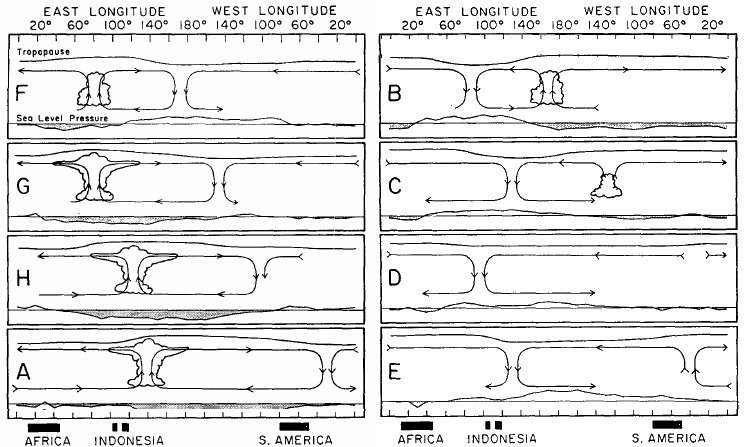
\includegraphics[width=0.7\textwidth]{figures/mjo_scheme.png}
    \caption{Эволюция состояния приэкваториальной атмосферы в течение типичного цикла КМД. Взято из \cite[Рис. 16]{Madden_Julian_1972}.}
    \label{fig:mjo_scheme}
\end{figure}

Принято описывать климатические моды с помощью специальных индексов, которые упрощают анализ данных явлений. Существует множество индексов, описывающих КМД, но наиболее распространенным является Real-time Multivariate MJO index (RMM), введенный в \cite{Wheeler_Hendon_2004}. Индекс RMM рассчитывается на основе потока уходящей длинноволновой излучения (outgoing longwave radiation, OLR) и скорости зонального ветра на 200 и 850 гПа (данные давления достигаются на высотах в 10--11 и 1--2 км соответственно). Набор трех таких переменных, взятых на широтно-долготной сетке 2.5\textdegree\texttimes2.5\textdegree, позволяет выделить паттерны, характерные для КМД, как в атмосферной циркуляции (которая характеризуется зональными ветрами), так и в глубокой конвекции (которая описывается OLR).

КМД всегда происходит совместно с климатической изменчивостью других временных и пространственных масштабов. Поэтому все три параметра, на основе которых рассчитывается КМД, сперва обрабатываются с целью удаления большей части изменчивости, не связанной с КМД. После этого производится меридиональное усреднение всех трех параметров по полосе 15\textdegree~с.~ш. -- 15\textdegree~ю.~ш., что приводит к тому, что для каждого дня получается три набора данных, каждый из которых обладает длиной 144. Такие три набора данных объединяются вместе и формируют 432-мерный вектор, для которого выделяются эмпирические ортогональные функции (ЭОФ). ЭОФ для физического процесса~---~такие взаимно ортогональные пространственные паттерны, рассчитываемые из данных, что с их помощью можно устроить разложение сложного процесса на относительно простые части. Первая ЭОФ выбирается таким образом, что объясняет наибольшую возможную часть дисперсии данных, вторая ЭОФ выбирается таким образом, что объясняет наибольшую возможную часть дисперсии оставшихся данных и так далее \cite[Гл. 6]{Zhang_et_al_2020} (более строго процесс вычисления ЭОФ будет описан в разделе \ref{sec:futher_analysis}). Временные коэффициенты для различных ЭОФ называются главными компонентами (ГК). Первые две ГК для вышеописанного набора данных составляют индекс RMM и обозначаются как RMM1 и RMM2.

Физически RMM1 описывает колебание конвекции над регионом, который далее будет называться Морским Континентом по аналогии с англоязычным устоявшимся термином Ma\-ri\-time Continent, под которым подразумевается обширный район (по долготе от 90\textdegree~в.~д. до 150\textdegree~в.~д. и по широте между 20\textdegree~с.~ш. и 10\textdegree~ю.~ш.) между Индийским и Тихим океаном, включающим Индонезийский архипелаг, острова Борнео, Новая Гвинея, Филиппинские острова и окружающие моря; RMM2 отвечает за колебание конвекции над Индийским океаном (см. рис. \ref{fig:wh04_fig1}). Принято иллюстрировать состояние КМД как точку на фазовой плоскости (RMM1, RMM2), которая изображена на рис. \ref{fig:rmm_diagram}, на котором отмечена стрелкой типичная траектория состояния КМД. На рис. \ref{fig:wh04_fig7} показаны реальные траектории состояний КМД на фазовой плоскости, видно, что они сильно изменчивы, но в среднем совпадают с движением по окружности.

\begin{figure}[t]  
    \centering
    \begin{subfigure}{.49\textwidth}
		\centering
		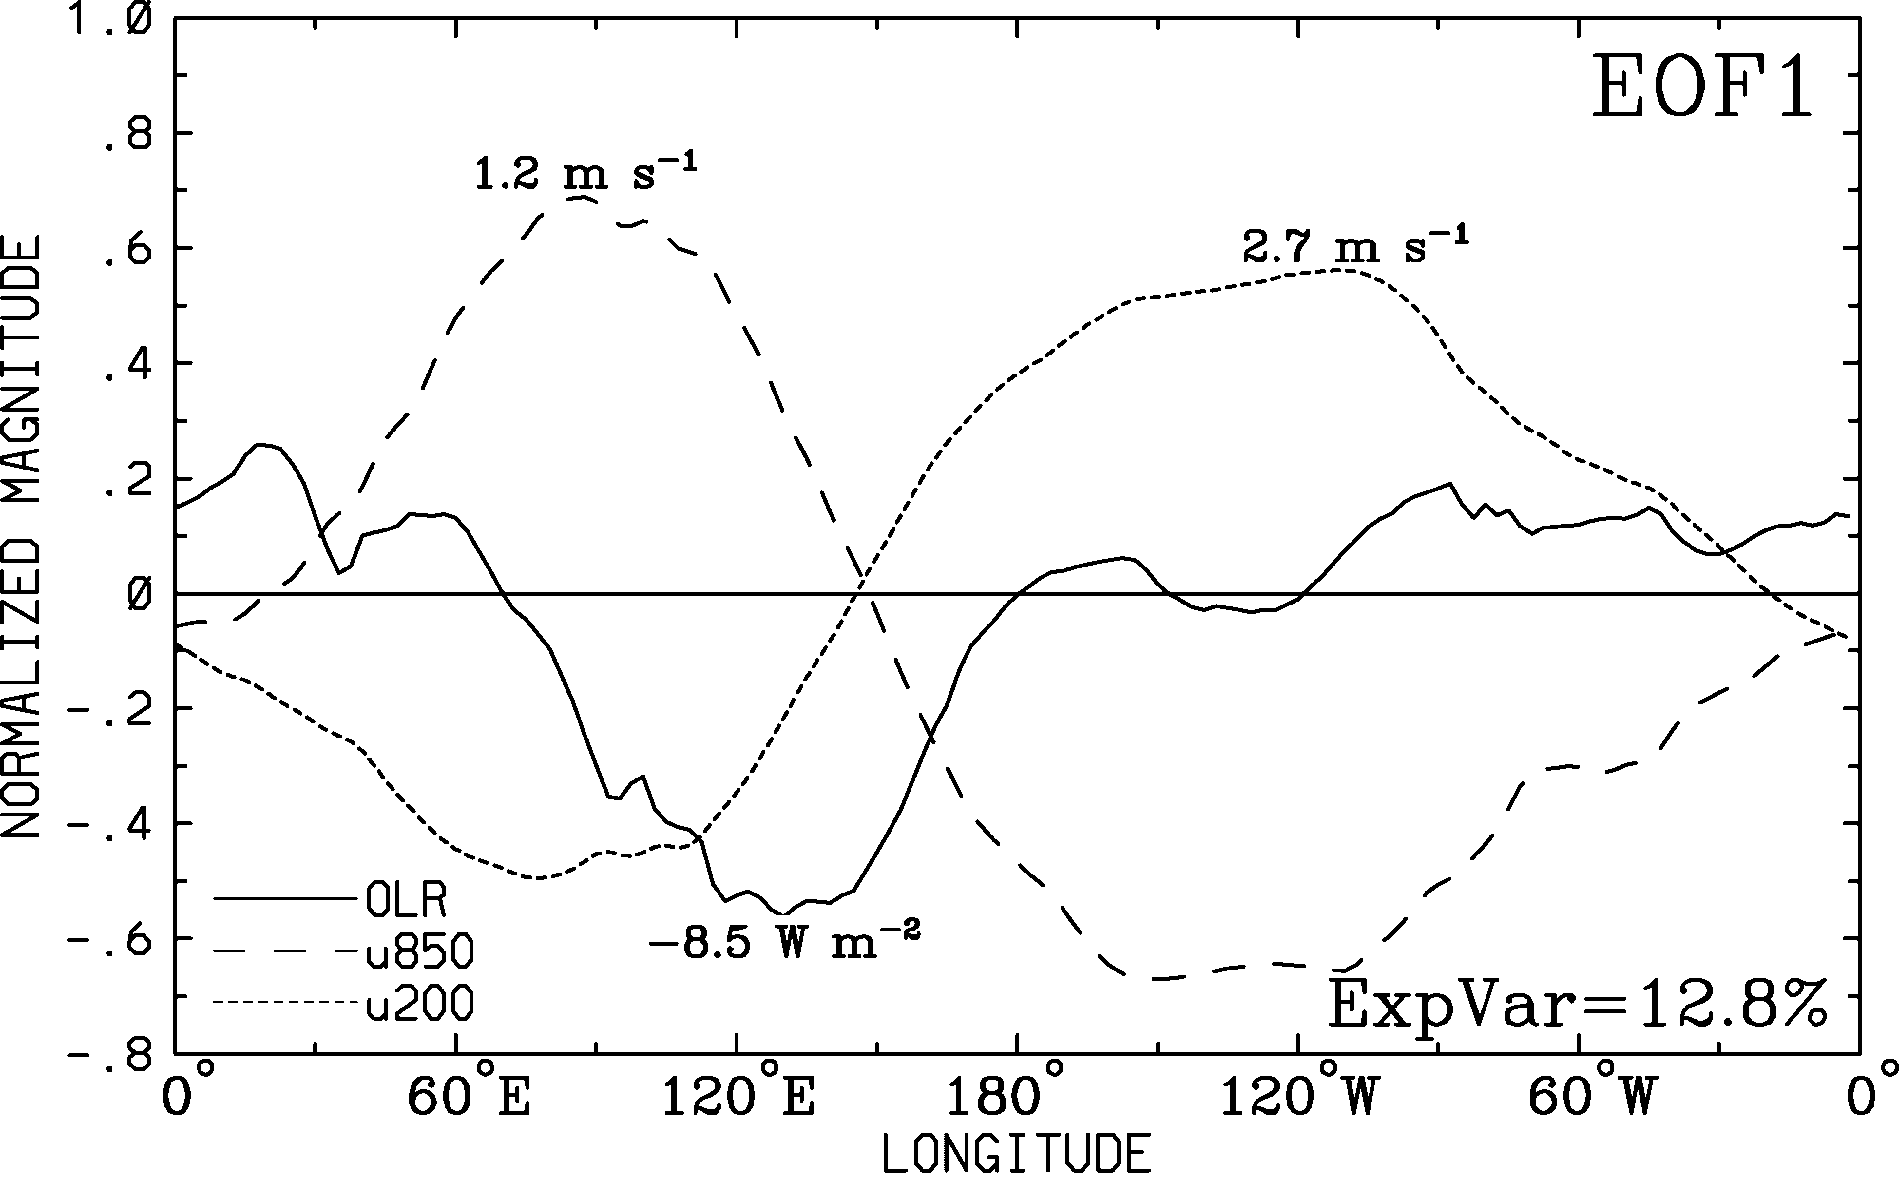
\includegraphics[width=\textwidth]{figures/wh04_fig1_eof1.png}
    \end{subfigure}
    \hfill
    \begin{subfigure}{.49\textwidth}
		\centering
		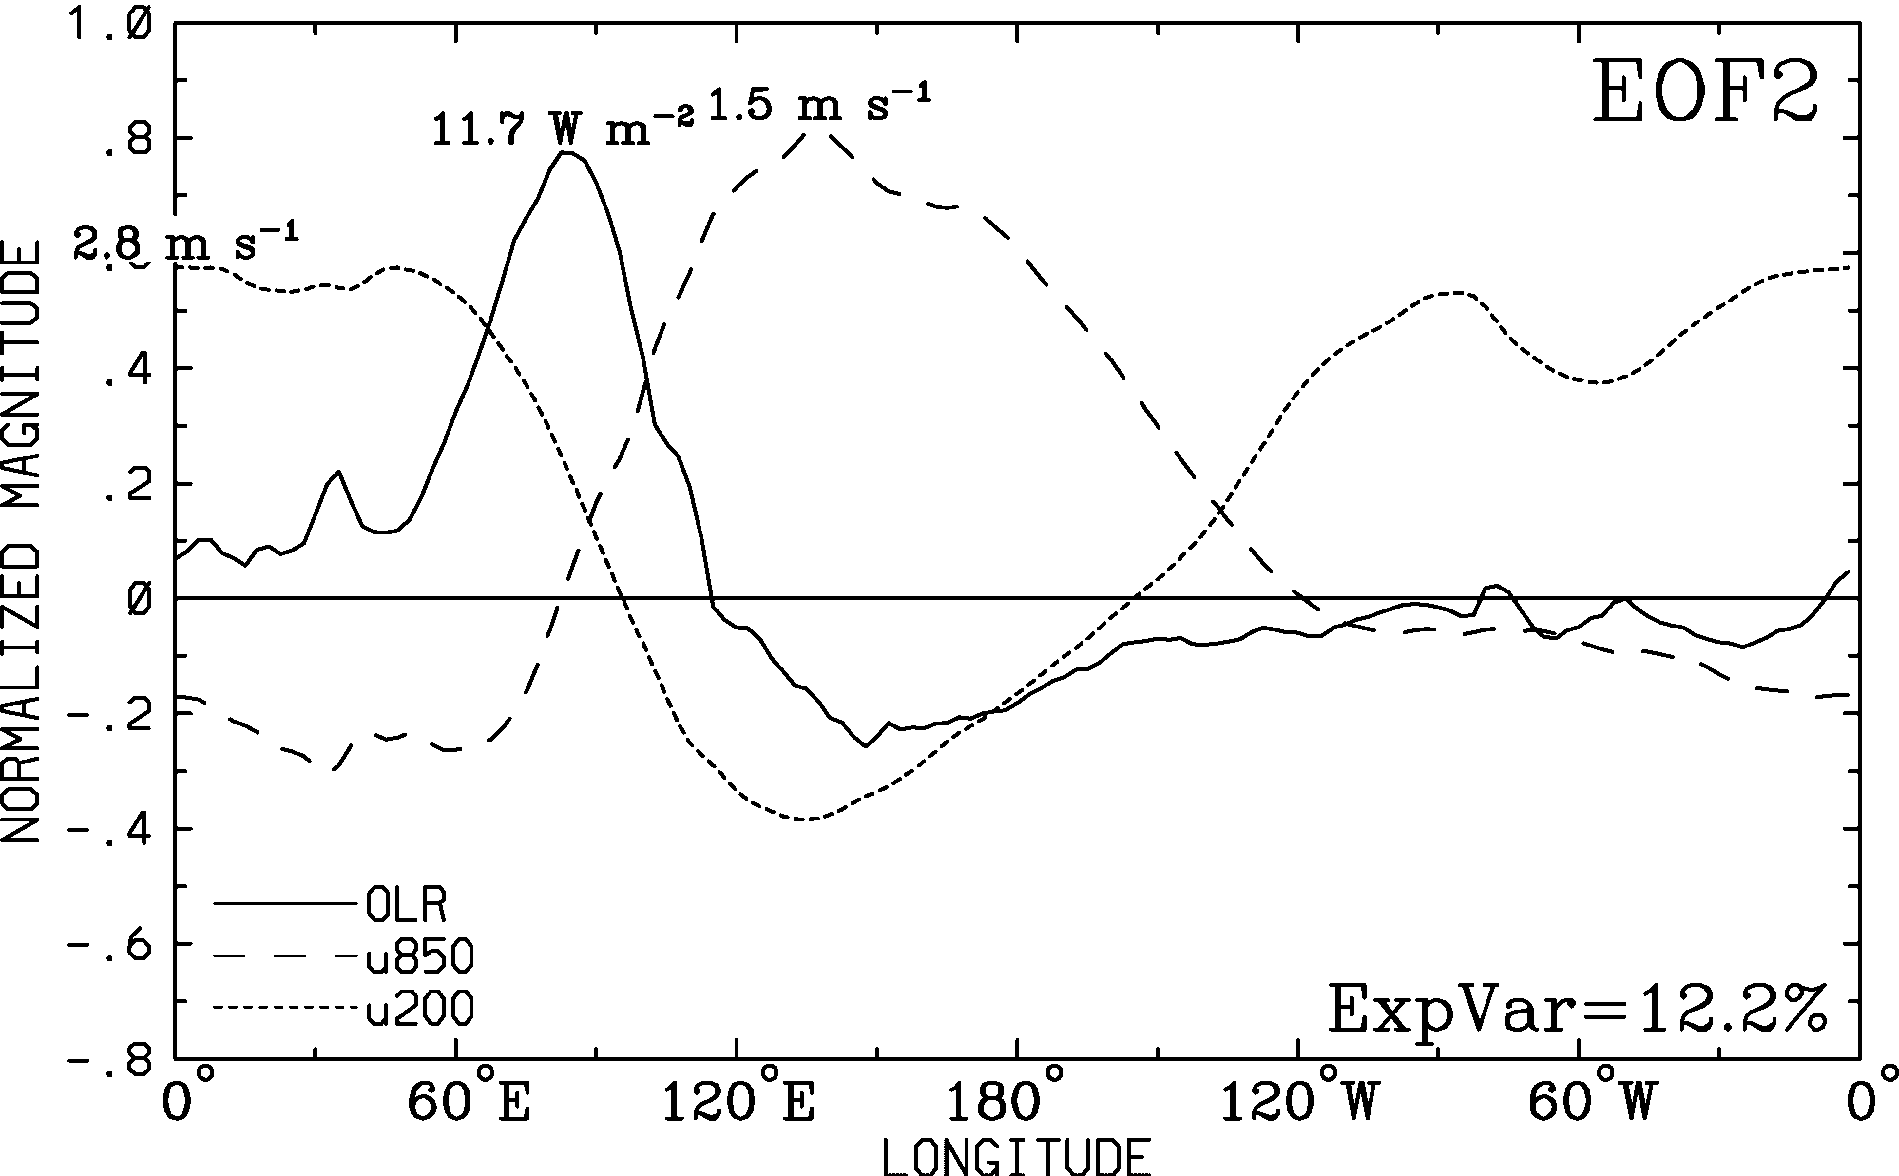
\includegraphics[width=\textwidth]{figures/wh04_fig1_eof2.png}
    \end{subfigure}
    \caption{Долготная структура первых двух ЭОФ, получаемых при вычислении индекса RMM. Непрерывные кривые обозначают OLR и описывают паттерны глубокой конвекции, характерные для КМД. Взято из \cite[рис. 1]{Wheeler_Hendon_2004}.}
	\label{fig:wh04_fig1}
\end{figure}

\begin{figure}
    \centering  
    \begin{subfigure}[tb]{.45\textwidth}
		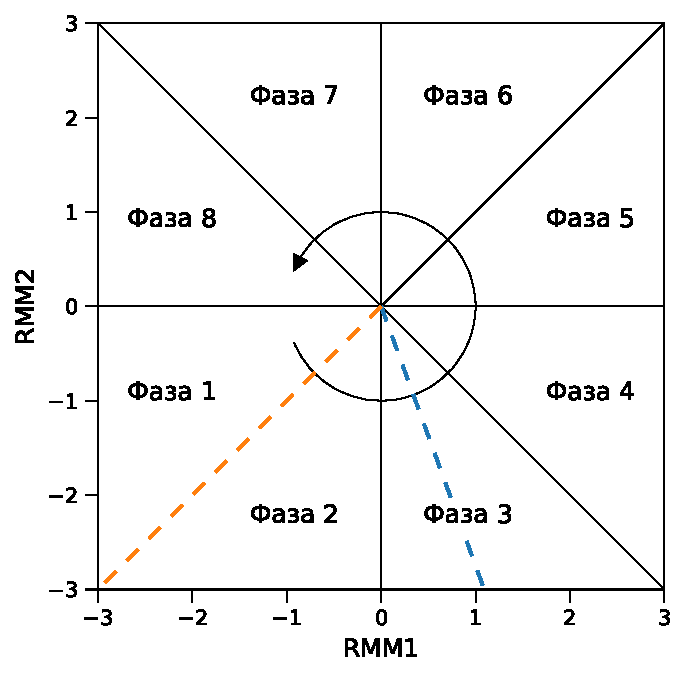
\includegraphics[width=\textwidth]{figures/rmm_diagram.pdf}
		\caption{}
		\label{fig:rmm_diagram}
	\end{subfigure}
	\hfill
	\begin{subfigure}[tb]{.45\textwidth}
		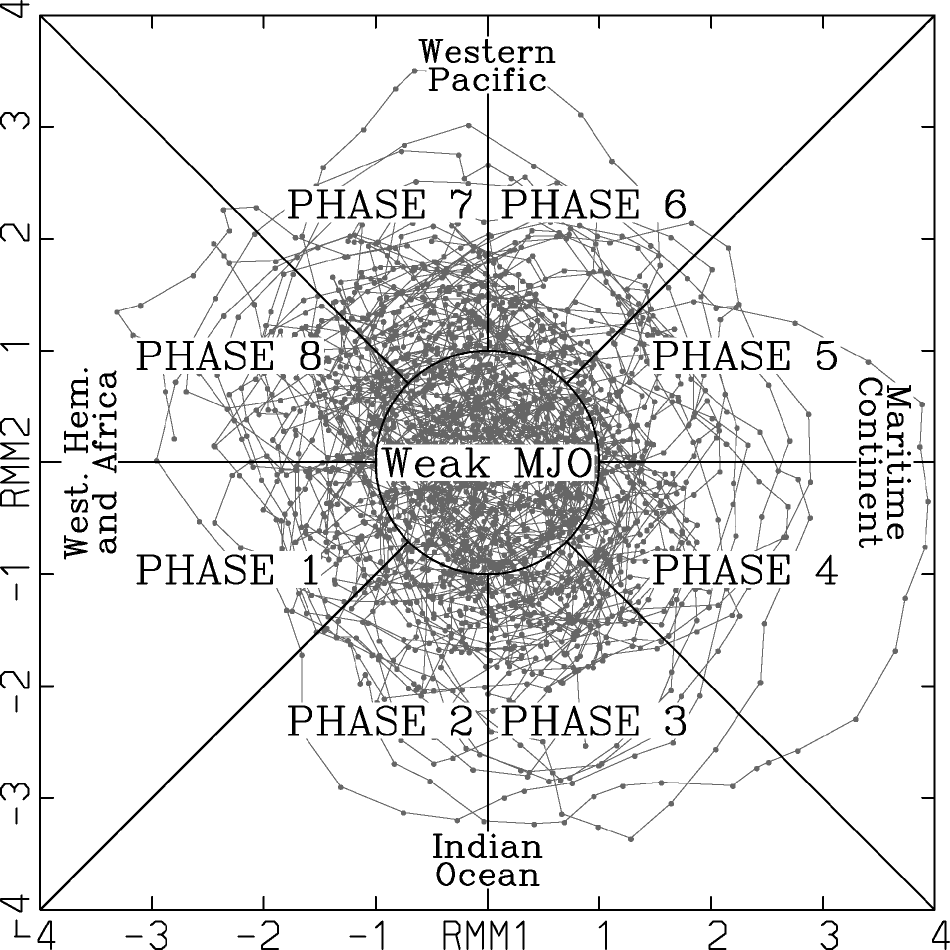
\includegraphics[width=\textwidth]{figures/wh04_fig7.png}
		\caption{}
		\label{fig:wh04_fig7}
	\end{subfigure}
    \caption{(a): Разбиение фазовой плоскости индекса RMM на восемь секторов, которые определяются как восемь фаз КМД. Закрученная стрелка схематично обозначает типичную траекторию точки в течение одного цикла КМД. Пунктирными линиями отмечены направления на плоскости (RMM1, RMM2), дающие наибольшую корреляцию с моделируемым ИП (голубая линия) и с измеренным в Антарктике в дни хорошей погоды ГП (оранжевая линия). (b): Траектория состояний КМД в зимние месяцы с 1974 по 2003 год на плоскости (RMM1, RMM2). Взято из \cite[рис. 7]{Wheeler_Hendon_2004}.}
    \label{fig:rmm_planes}
\end{figure}

При исследовании КМД исторически выделяют восемь так называемых фаз КМД. Технически такие фазы определяются как восемь секторов плоскости (RMM1, RMM2) с углом раствора сектора 45\textdegree, нумеруют такие сектора против часовой стрелки, начиная с направления отрицательного RMM1 (см. рис. \ref{fig:rmm_diagram}). Физически данные восемь фаз КМД следует понимать как восемь характерных состояний КМД, каждому из которых отвечает свойственное данной фазе распределение конвективной активности и структура циркуляции. Распределение конвективной активности в каждую из фаз КМД можно проиллюстрировать с помощью рис. \ref{fig:map_of_olr_anomaly}, где приведено распределение OLR. Следует понимать, что положительная аномалия OLR отвечает уменьшению конвективной активности, а отрицательная~---~увеличению, так как при увеличении конвективной активности начинается формирование облаков, которые поглощают значительную часть излучения от Земли и тем самым ослабляют OLR. Из рис. \ref{fig:map_of_olr_anomaly} видно, что с увеличением номера фазы КМД область усиленной конвективной активности и область ослабленной конвективной активности сносятся друг за другом на восток.

\begin{figure}[tb]
	\centering
	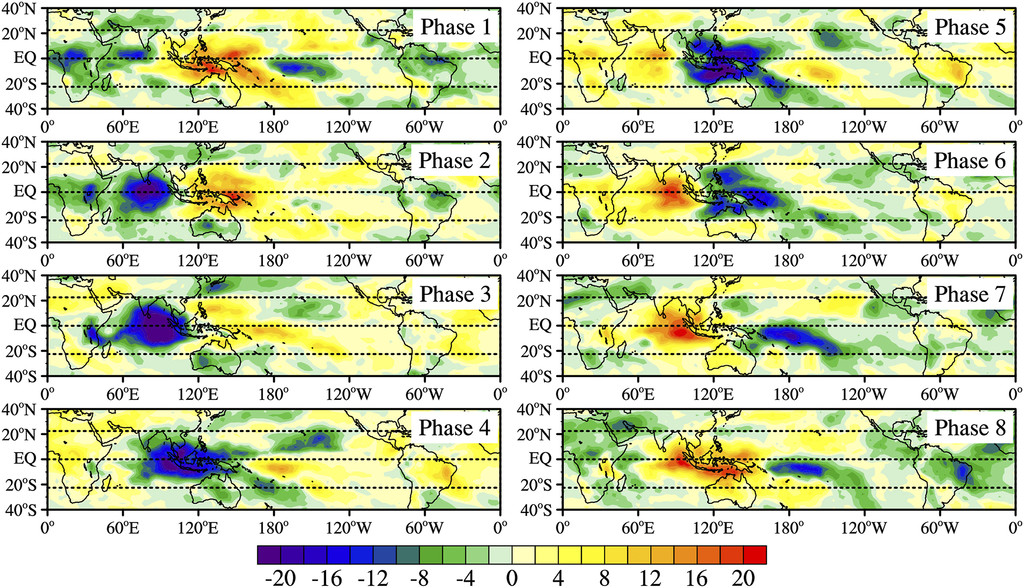
\includegraphics[width=\textwidth]{figures/map_of_olr_anomaly.jpg}
	\caption{Аномалии OLR ($\textnormal{Вт}/\textnormal{м}^2$) в течение каждой из фаз КМД за месяца зимы в северном полушарии. Взяты лишь дни с амплитудой индекса RMM больше 1. Позаимствовано из \cite{Wang_et_al_2018}.}
	\label{fig:map_of_olr_anomaly}
\end{figure}

В настоящем работе используются данные индекса RMM за период 1980--2020 годов, которые были взяты с веб-сайта Австралийского бюро метеорологии (\url{http://www.bom.gov.au/climate/mjo /}).
